\section{Definition}
\vspace{0.2in}
\hspace*{0.16in}

A blood cell, also called a hematopoietic cell, hemocyte, or hematocyte, is a cell produced through hematopoiesis and found mainly in the blood. Major types of blood cells include red blood cells (erythrocytes), white blood cells (leukocytes), and platelets (thrombocytes). Together, these three kinds of blood cells add up to a total 45\% of the blood tissue by volume, with the remaining 55\% of the volume composed of plasma, the liquid component of blood. \textsuperscript{\cite{hopkins1993human}}\\

\vspace{0.1in}

\begin{figure}[h]
\centering
  \vspace{-0.1in}
    \centerline{\fbox{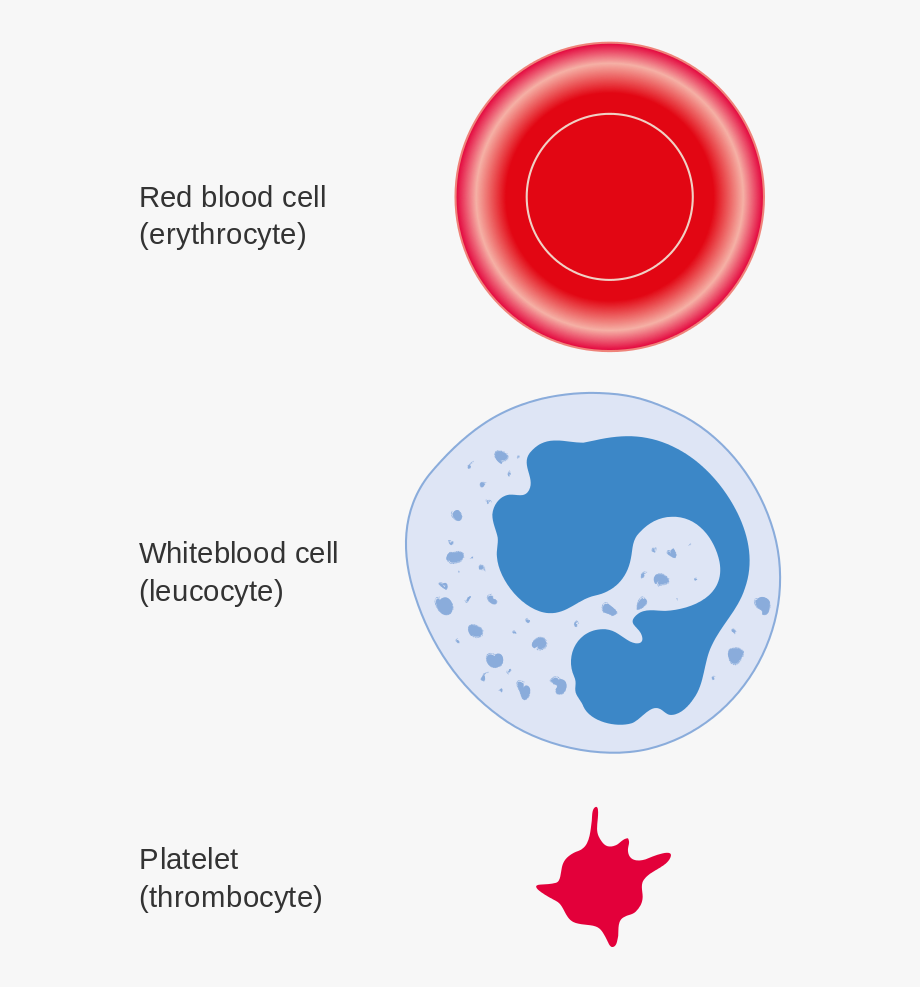
\includegraphics[width = 3in, height = 3in]{../images/blood_cells.png}}}
    \caption{Blood cells}
\end{figure}

That said, there are three main types of blood cells:

\subsection{Red Blood Cells}

Red blood cells (RBCs) are the cells which carry fresh oxygen all over the human body. This is important to our health. They are round with a flattish, indented center, like doughnuts without a hole. 
The hemoglobin is the protein found inside the red blood cell, and it's main purpose is carrying oxygen.

Most people don't think about their red blood cells unless they have a disease that affects these cells. Problems with red blood cells can be caused by illnesses or a lack of iron or vitamins. Some diseases of the red blood cells are inherited.

Diseases of the red blood cells include many types of anemia. This is a condition in which there are too few red blood cells to carry enough oxygen all over the body. People with anemia may have red blood cells that have an abnormal shape or that look normal, larger than normal, or smaller than normal.

Symptoms of anemia include tiredness, fast heart rate, pale skin, feeling cold, and, in severe cases, heart failure. Children who don't have enough healthy red blood cells grow and develop more slowly than other children. These symptoms show how important red blood cells are to your daily life. \textsuperscript{\cite{Department_2022_rochester}}

\subsection{White Blood Cells}

On the other hand, White Blood Cells (WBCs), also known as leukocytes, are the ones responsible for protecting the human body from infections. As part of the immune system, These cells circulate in the blood and respond to injury or illness. They travel through the bloodstream searching for infections. Then, they notify other WBCs of their location to help defending against attacks from other unknown organisms. Once the army of WBCs arrive, they fight the invader by producing antibody proteins to attach to the organism and destroy it. \textsuperscript{\cite{Attacking_Any_Unknown_2022_clevelandclinic}}

White Blood Cells are divided into five types:

\begin{itemize}
  \item \textbf{Neutrophils:} Help protect your body from infections by killing bacteria, fungi and foreign debris.
  \item \textbf{Lymphocytes:} Consist of T cells, natural killer cells and B cells to protect against viral infections and produce proteins to help you fight infection (antibodies).
  \item \textbf{Eosinophils:} Identify and destroy parasites, cancer cells and assists basophils with your allergic response.
  \item \textbf{Basophils:} Produces an allergic response like coughing, sneezing or a runny nose.
  \item \textbf{Monocytes:} Defend against infection by cleaning up damaged cells.
\end{itemize}

\subsection{Platelets}
